%iffalse
\let\negmedspace\undefined
\let\negthickspace\undefined
\documentclass[journal,12pt,twocolumn]{IEEEtran}
\usepackage{cite}
\usepackage{amsmath,amssymb,amsfonts}
\usepackage{graphicx}
\usepackage{textcomp}
\usepackage{xcolor}
\usepackage{txfonts}
\usepackage{listings}
\usepackage{enumitem}
\usepackage{mathtools}
\usepackage{gensymb}
\usepackage{comment}
\usepackage[breaklinks=true]{hyperref}
\usepackage{tkz-euclide} 
\usepackage{listings}
\usepackage{gvv}                                        
\def\inputGnumericTable{}                                 
\usepackage[latin1]{inputenc}                                
\usepackage{color}                                            
\usepackage{array}                                            
\usepackage{longtable}                                       
\usepackage{calc}                                             
\usepackage{multirow}                                         
\usepackage{hhline}                                           
\usepackage{ifthen}                                           
\usepackage{lscape}
\usepackage[export]{adjustbox}

\newtheorem{theorem}{Theorem}[section]
\newtheorem{problem}{Problem}
\newtheorem{proposition}{Proposition}[section]
\newtheorem{lemma}{Lemma}[section]
\newtheorem{corollary}[theorem]{Corollary}
\newtheorem{example}{Example}[section]
\newtheorem{definition}[problem]{Definition}
\newcommand{\BEQA}{\begin{eqnarray}}
\newcommand{\EEQA}{\end{eqnarray}}
\newcommand{\define}{\stackrel{\triangle}{=}}
\newtheorem{rem}{Remark}

\begin{document}
\parindent 0px
\bibliographystyle{IEEEtran}

\vspace{3cm}

\title{}
\author{EE23BTECH11217 - Prajwal M$^{*}$
}
\maketitle
\newpage
\bigskip

\renewcommand{\thefigure}{\theenumi}
\renewcommand{\thetable}{\theenumi}

\section*{Exercise 9.5}
\noindent25) \hspace{2pt} \textbf{Find the sum of the following series up to n terms and obtain the Z-transform:}
$$ 
\ldots + 0 + \frac{1^3}{1} + \frac{1^3 + 2^3}{1 + 3} + \frac{1^3 + 2^3 + 3^3}{1 + 3 + 5} + \ldots$$

\noindent Solution: 

\begin{align}
    x\brak{n} & = \frac{\sum_{i=0}^{n} \brak{i+1}^{3}}{\sum_{j=0}^{n} \brak{2j+1}} u\brak{n}  \\
    & = \frac{\brak{n+1}^{3} * u\brak{n}}{\brak{2n+1} * u\brak{n}}u\brak{n}\\
    & = \frac{\mathcal{Z}^{-1}\cbrak{\mathcal{Z}\cbrak{\brak{n+1}^{3}}\mathcal{Z}\cbrak{u\brak{n}}}}{\mathcal{Z}^{-1}\cbrak{\mathcal{Z}\cbrak{{2n+1}} \mathcal{Z}\cbrak{u\brak{n}}}} u\brak{n}\\
    & = \frac{\mathcal{Z}^{-1}\cbrak{\brak{\frac{z^4+4z^3+z^2}{\brak{z-1}^4}}\brak{\frac{z}{z-1}}}}{\mathcal{Z}^{-1}\cbrak{ \brak{\frac{z^2 + z}{\brak{z-1}^2}}\brak{\frac{z}{z-1}}}} u\brak{n}\\
    & = \frac{\frac{1}{2\pi j} \oint_C  \cbrak{\brak{\frac{z^5+4z^4+z^3}{\brak{z-1}^5}}z^{n-1}} dz}{\frac{1}{2\pi j} \oint_C  \cbrak{ \brak{\frac{z^3 + z^2}{\brak{z-1}^3}}z^{n-1}} dz}u\brak{n}\\
    & = \frac{\frac{1}{4!} \lim_{n\rightarrow1}{\frac{d^4}{dz^4} \cbrak{z^{n+4}+4z^{n+3}+z^{n+2}}}}{\frac{1}{2!} \lim_{n\rightarrow1}{\frac{d^2}{dz^2} \cbrak{z^{n+2}+z^{n+1}}}}u\brak{n}\\
    & = \frac{\brak{n + 2}^{2}}{4} u\brak{n} \label{x(n)}
\end{align}
\begin{align}
    s\brak{n} & = \sum_{r=-\infty}^{n} x\brak{r}\\
    \notag \text{using \eqref{x(n)}, } \\
    s\brak{n} & = \sum_{r=-\infty}^{n} \frac{\brak{r+2}^{2}}{4} u\brak{r} \\
    & = \sum_{r=0}^{n}\frac{r^2 + 4r + 4}{4} \\
    & = 1 + \frac{37n}{24} + \frac{5n^2}{8} + \frac{n^3}{12}\\
    & = \frac{\brak{n+2}^2}{4} u\brak{n}* u\brak{n}\\
    & = \mathcal{Z}^{-1}\cbrak{\frac{z \brak{1 - 3 z + 4 z^2}}{4 (z - 1)^3}\frac{z}{z-1}}\\
    & = \frac{1}{2\pi j} \oint_C  \cbrak{\brak{\frac{4z^4-3z^3 + z^2}{4\brak{z-1}^4}}z^{n-1}} dz\\
    & = \frac{1}{3!} \lim_{n\rightarrow1}{\frac{d^3}{dz^3} \cbrak{z^{n+3}-\frac{3z^{n+2}}{4}+\frac{z^{n+1}}{4}}}\\
    & = 1 + \frac{37n}{24} + \frac{5n^2}{8} + \frac{n^3}{12}
\end{align}

\begin{figure}[h]
   \centering
   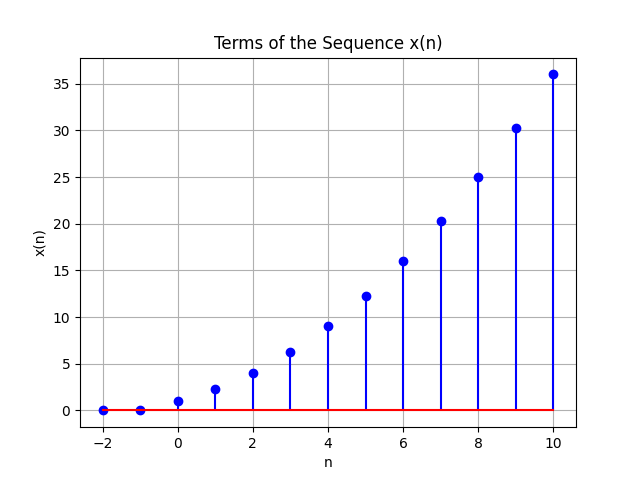
\includegraphics[width=1\columnwidth]{figs/plot.png}
   \caption{Plot of x(n) vs n}
   \label {fig: 11.9.5.25.1}
\end{figure}

\begin{table}[h]
    \centering
    
\begin{table}[h]
  \centering
  \begin{tabular}{|c|c|}
    \hline
    	\textbf{Symbol} & \textbf{Parameters} \\
    \hline
	  x(n) & general term of the series \\
    \hline
	  $X$(z) & Z-transform of x(n) \\
    \hline 
	  u(n) & unit step function \\
    \hline
  \end{tabular}
  \vspace{0.3cm}
  \caption{Parameters}
  \label{tab:parameters}
\end{table}

    \caption{Parameters}
    \label{tab: 11.9.5.25.1}
\end{table}

\end{document}

